% ============================================================================
% CHƯƠNG 7: QUICK SORT SONG SONG
% ============================================================================
\chapter{Quick Sort Song song}
\label{chap:quicksort}

\section{Giới thiệu Quick Sort}

\subsection{Thuật toán tuần tự}

Quick Sort là thuật toán sắp xếp chia để trị (divide-and-conquer) với độ phức tạp trung bình $O(n \log n)$ và worst-case $O(n^2)$. Thuật toán gồm 3 bước:

\begin{enumerate}
    \item \textbf{Chọn pivot}: Chọn một phần tử làm mốc
    \item \textbf{Partition}: Chia mảng thành 2 phần: nhỏ hơn pivot và lớn hơn pivot
    \item \textbf{Đệ quy}: Áp dụng Quick Sort cho 2 phần
\end{enumerate}

\begin{figure}[H]
\centering
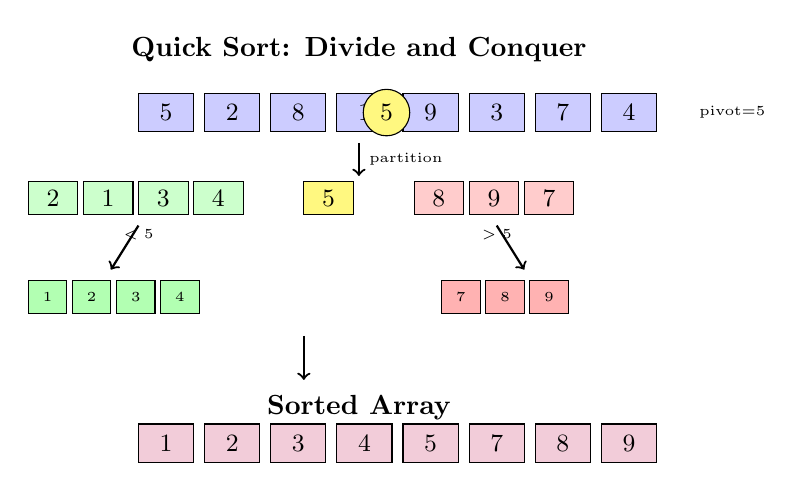
\begin{tikzpicture}[scale=0.7]
    % Level 0: Original
    \node[font=\bfseries] at (6, 9) {Quick Sort: Divide and Conquer};
    
    \foreach \i/\v in {0/5, 1/2, 2/8, 3/1, 4/9, 5/3, 6/7, 7/4} {
        \draw[fill=blue!20] ({\i*1.2+2}, 7.5) rectangle ++(1, 0.7);
        \node[font=\small] at ({\i*1.2+2.5}, 7.85) {\v};
    }
    \node[draw, circle, fill=yellow!50, font=\small] at (6.5, 7.85) {5};
    \node[right, font=\tiny] at (12, 7.85) {pivot=5};
    
    % Arrow
    \draw[->, thick] (6, 7.3) -- (6, 6.7) node[midway, right, font=\tiny] {partition};
    
    % Level 1: After partition
    % Left partition (< 5)
    \foreach \i/\v in {0/2, 1/1, 2/3, 3/4} {
        \draw[fill=green!20] (\i*1, 6) rectangle ++(0.9, 0.6);
        \node[font=\small] at ({\i*1+0.45}, 6.3) {\v};
    }
    \node[below, font=\tiny] at (2, 5.9) {$< 5$};
    
    % Pivot
    \draw[fill=yellow!50] (5, 6) rectangle ++(0.9, 0.6);
    \node[font=\small] at (5.45, 6.3) {5};
    
    % Right partition (> 5)
    \foreach \i/\v in {0/8, 1/9, 2/7} {
        \draw[fill=red!20] ({7+\i*1}, 6) rectangle ++(0.9, 0.6);
        \node[font=\small] at ({7+\i*1+0.45}, 6.3) {\v};
    }
    \node[below, font=\tiny] at (8.5, 5.9) {$> 5$};
    
    % Arrows to Level 2
    \draw[->, thick] (2, 5.8) -- (1.5, 5);
    \draw[->, thick] (8.5, 5.8) -- (9, 5);
    
    % Level 2: Recursive
    % Left sub-array
    \foreach \i/\v in {0/1, 1/2, 2/3, 3/4} {
        \draw[fill=green!30] ({\i*0.8}, 4.2) rectangle ++(0.7, 0.6);
        \node[font=\tiny] at ({\i*0.8+0.35}, 4.5) {\v};
    }
    
    % Right sub-array
    \foreach \i/\v in {0/7, 1/8, 2/9} {
        \draw[fill=red!30] ({7.5+\i*0.8}, 4.2) rectangle ++(0.7, 0.6);
        \node[font=\tiny] at ({7.5+\i*0.8+0.35}, 4.5) {\v};
    }
    
    % Final sorted
    \draw[->, thick] (5, 3.8) -- (5, 3);
    \node[font=\bfseries] at (6, 2.5) {Sorted Array};
    \foreach \i/\v in {0/1, 1/2, 2/3, 3/4, 4/5, 5/7, 6/8, 7/9} {
        \draw[fill=purple!20] ({\i*1.2+2}, 1.5) rectangle ++(1, 0.7);
        \node[font=\small] at ({\i*1.2+2.5}, 1.85) {\v};
    }
    
\end{tikzpicture}
\caption{Minh họa thuật toán Quick Sort}
\label{fig:quicksort_overview}
\end{figure}

\section{Song song hóa Quick Sort}

\subsection{Thách thức}

Song song hóa Quick Sort trên GPU gặp nhiều thách thức:

\begin{enumerate}
    \item \textbf{Đệ quy}: GPU không hỗ trợ đệ quy sâu hiệu quả
    \item \textbf{Load imbalance}: Partition có thể không đều
    \item \textbf{Dynamic parallelism}: Số task thay đổi theo mỗi level
    \item \textbf{Small segments}: Overhead lớn khi sort các đoạn nhỏ
\end{enumerate}

\subsection{Chiến lược GPU Quick Sort}

\begin{figure}[H]
\centering
\begin{tikzpicture}[scale=0.75]
    % GPU Strategy
    \node[font=\bfseries] at (5, 7) {Chiến lược GPU Quick Sort};
    
    % Phase 1: Large segments
    \draw[fill=blue!10, rounded corners] (-0.5, 4.5) rectangle (4.5, 6.5);
    \node[font=\bfseries, blue] at (2, 6) {Phase 1: Global Partition};
    \node[font=\small, align=center] at (2, 5.2) {Segments lớn\\GPU parallel partition\\Dynamic parallelism};
    
    % Phase 2: Medium segments
    \draw[fill=green!10, rounded corners] (5.5, 4.5) rectangle (10.5, 6.5);
    \node[font=\bfseries, green!50!black] at (8, 6) {Phase 2: Block-level};
    \node[font=\small, align=center] at (8, 5.2) {Mỗi block sort\\một segment\\Shared memory};
    
    % Phase 3: Small segments
    \draw[fill=orange!10, rounded corners] (2.5, 2) rectangle (7.5, 4);
    \node[font=\bfseries, orange!70!black] at (5, 3.5) {Phase 3: Warp/Thread Sort};
    \node[font=\small, align=center] at (5, 2.7) {Insertion sort\\hoặc sorting network\\cho segments nhỏ ($<32$)};
    
    % Arrows
    \draw[->, very thick] (2, 4.4) -- (5, 4.1);
    \draw[->, very thick] (8, 4.4) -- (5, 4.1);
    
    % Size indicators
    \node[font=\tiny, right] at (4.5, 5.5) {$n > 1024$};
    \node[font=\tiny, left] at (5.5, 5.5) {$32 < n < 1024$};
    \node[font=\tiny] at (5, 1.6) {$n \leq 32$};
    
\end{tikzpicture}
\caption{Chiến lược phân tầng cho GPU Quick Sort}
\label{fig:gpu_quicksort_strategy}
\end{figure}

\section{Thuật toán Parallel Partition}

\subsection{Work-Efficient Partition}

Parallel partition là bước quan trọng nhất, sử dụng kỹ thuật \textbf{filter} với prefix sum:

\begin{lstlisting}[caption={Parallel Partition với Prefix Sum}, label={lst:parallel_partition}]
// Buoc 1: Moi thread danh dau phan tu < pivot
__global__ void markSmaller(int *data, int *flags, int pivot, int n) {
    int idx = blockIdx.x * blockDim.x + threadIdx.x;
    if (idx < n) {
        flags[idx] = (data[idx] < pivot) ? 1 : 0;
    }
}

// Buoc 2: Exclusive Prefix Sum tren flags
// (su dung thrust hoac tu cai dat)

// Buoc 3: Scatter dua tren prefix sum
__global__ void scatterPartition(int *input, int *output, 
                                  int *prefixSum, int *flags, 
                                  int pivot, int n, int numSmaller) {
    int idx = blockIdx.x * blockDim.x + threadIdx.x;
    if (idx < n) {
        int value = input[idx];
        int pos;
        if (flags[idx]) {
            // Phan tu < pivot: dat vao vi tri prefixSum[idx]
            pos = prefixSum[idx];
        } else {
            // Phan tu >= pivot: dat vao vi tri numSmaller + (idx - prefixSum[idx])
            pos = numSmaller + (idx - prefixSum[idx]);
        }
        output[pos] = value;
    }
}
\end{lstlisting}

\begin{figure}[H]
\centering
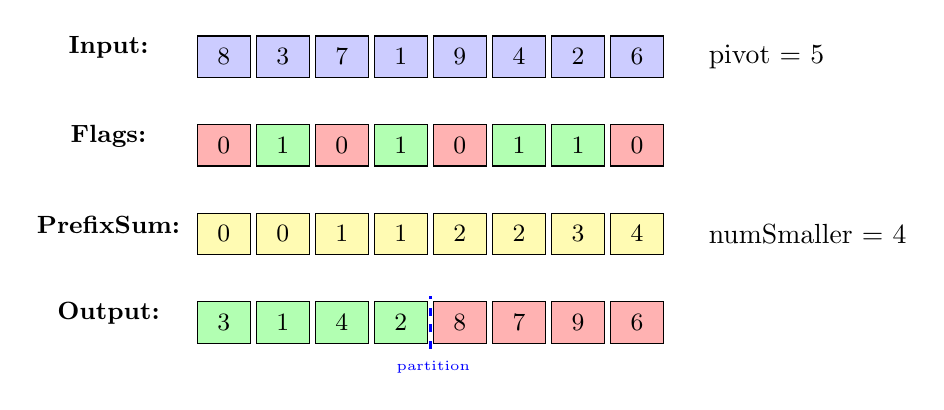
\begin{tikzpicture}[scale=0.75]
    % Input
    \node[font=\small\bfseries] at (-1.5, 6) {Input:};
    \foreach \i/\v in {0/8, 1/3, 2/7, 3/1, 4/9, 5/4, 6/2, 7/6} {
        \draw[fill=blue!20] (\i, 5.5) rectangle ++(0.9, 0.7);
        \node[font=\small] at ({\i+0.45}, 5.85) {\v};
    }
    \node[right] at (8.5, 5.85) {pivot = 5};
    
    % Flags
    \node[font=\small\bfseries] at (-1.5, 4.5) {Flags:};
    \foreach \i/\v in {0/0, 1/1, 2/0, 3/1, 4/0, 5/1, 6/1, 7/0} {
        \pgfmathsetmacro{\col}{\v == 1 ? "green!30" : "red!30"}
        \draw[fill=\col] (\i, 4) rectangle ++(0.9, 0.7);
        \node[font=\small] at ({\i+0.45}, 4.35) {\v};
    }
    
    % Prefix Sum
    \node[font=\small\bfseries] at (-1.5, 3) {PrefixSum:};
    \foreach \i/\v in {0/0, 1/0, 2/1, 3/1, 4/2, 5/2, 6/3, 7/4} {
        \draw[fill=yellow!30] (\i, 2.5) rectangle ++(0.9, 0.7);
        \node[font=\small] at ({\i+0.45}, 2.85) {\v};
    }
    \node[right] at (8.5, 2.85) {numSmaller = 4};
    
    % Output
    \node[font=\small\bfseries] at (-1.5, 1.5) {Output:};
    \foreach \i/\v in {0/3, 1/1, 2/4, 3/2, 4/8, 5/7, 6/9, 7/6} {
        \pgfmathsetmacro{\col}{\i < 4 ? "green!30" : "red!30"}
        \draw[fill=\col] (\i, 1) rectangle ++(0.9, 0.7);
        \node[font=\small] at ({\i+0.45}, 1.35) {\v};
    }
    
    % Separator
    \draw[very thick, dashed, blue] (3.95, 0.9) -- (3.95, 1.8);
    \node[font=\tiny, blue] at (4, 0.6) {partition};
    
\end{tikzpicture}
\caption{Parallel Partition với Prefix Sum}
\label{fig:parallel_partition}
\end{figure}

\section{GPU Quick Sort Implementation}

\subsection{Dynamic Parallelism Approach}

CUDA Dynamic Parallelism cho phép kernel launch kernel khác, phù hợp cho Quick Sort:

\begin{lstlisting}[caption={Quick Sort với Dynamic Parallelism}, label={lst:quicksort_dynamic}]
#define THRESHOLD 32  // Nguong chuyen sang insertion sort

__device__ void insertionSort(int *data, int left, int right) {
    for (int i = left + 1; i <= right; i++) {
        int key = data[i];
        int j = i - 1;
        while (j >= left && data[j] > key) {
            data[j + 1] = data[j];
            j--;
        }
        data[j + 1] = key;
    }
}

__global__ void quickSortKernel(int *data, int left, int right) {
    if (right - left < THRESHOLD) {
        // Segment nho: dung insertion sort
        if (threadIdx.x == 0 && blockIdx.x == 0) {
            insertionSort(data, left, right);
        }
        return;
    }
    
    // Chon pivot (median-of-three)
    int mid = (left + right) / 2;
    int pivot = data[mid];
    
    // Parallel partition
    __shared__ int pivotPos;
    
    // ... (partition code) ...
    
    // De quy voi Dynamic Parallelism
    if (threadIdx.x == 0 && blockIdx.x == 0) {
        if (pivotPos > left) {
            quickSortKernel<<<1, 256>>>(data, left, pivotPos - 1);
        }
        if (pivotPos < right) {
            quickSortKernel<<<1, 256>>>(data, pivotPos + 1, right);
        }
        cudaDeviceSynchronize();
    }
}
\end{lstlisting}

\subsection{Block-level Quick Sort với Shared Memory}

\begin{lstlisting}[caption={Block Quick Sort với Shared Memory}, label={lst:block_quicksort}]
#define BLOCK_SIZE 256

__global__ void blockQuickSort(int *data, int n) {
    __shared__ int sharedData[BLOCK_SIZE];
    __shared__ int stack[64];  // Stack cho de quy
    __shared__ int top;
    
    int tid = threadIdx.x;
    int idx = blockIdx.x * blockDim.x + threadIdx.x;
    
    // Load data vao shared memory
    if (idx < n) {
        sharedData[tid] = data[idx];
    }
    __syncthreads();
    
    // Khoi tao stack
    if (tid == 0) {
        top = 0;
        stack[top++] = 0;
        stack[top++] = min(BLOCK_SIZE - 1, n - blockIdx.x * BLOCK_SIZE - 1);
    }
    __syncthreads();
    
    // Iterative quick sort voi stack
    while (top > 0) {
        __shared__ int left, right, pivot, pivotIdx;
        
        if (tid == 0) {
            right = stack[--top];
            left = stack[--top];
            pivotIdx = (left + right) / 2;
            pivot = sharedData[pivotIdx];
        }
        __syncthreads();
        
        if (right - left < 16) {
            // Small segment: insertion sort
            if (tid == 0) {
                insertionSort(sharedData, left, right);
            }
        } else {
            // Parallel partition trong shared memory
            // ... (partition logic) ...
        }
        __syncthreads();
    }
    
    // Ghi ket qua ve global memory
    if (idx < n) {
        data[idx] = sharedData[tid];
    }
}
\end{lstlisting}

\section{Bitonic Sort Network}

Cho các segment nhỏ, có thể dùng \textbf{Bitonic Sort} - một sorting network hiệu quả trên GPU:

\begin{figure}[H]
\centering
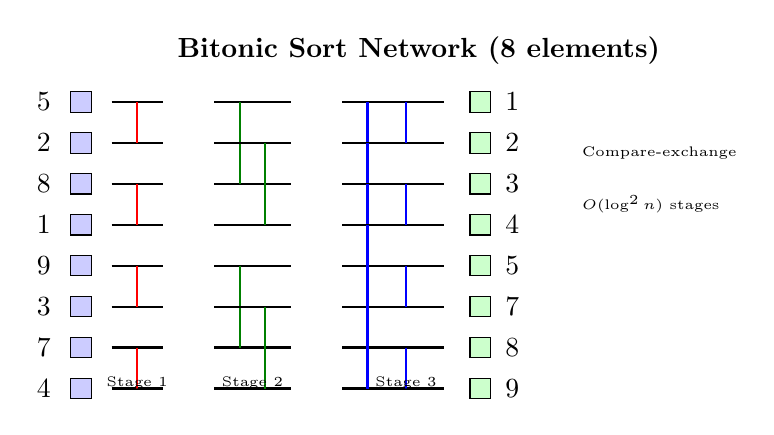
\begin{tikzpicture}[scale=0.65]
    \node[font=\bfseries] at (7, 7) {Bitonic Sort Network (8 elements)};
    
    % Input values
    \foreach \i/\v in {0/5, 1/2, 2/8, 3/1, 4/9, 5/3, 6/7, 7/4} {
        \node[left] at (0, {6-\i*0.8}) {\v};
        \draw[fill=blue!20] (0.2, {5.8-\i*0.8}) rectangle ++(0.4, 0.4);
    }
    
    % Stage 1: pairs
    \foreach \i in {0,2,4,6} {
        \draw[thick] (1, {6-\i*0.8}) -- (2, {6-\i*0.8});
        \draw[thick] (1, {6-(\i+1)*0.8}) -- (2, {6-(\i+1)*0.8});
        \draw[thick, red] (1.5, {6-\i*0.8}) -- (1.5, {6-(\i+1)*0.8});
    }
    \node[font=\tiny] at (1.5, 0.5) {Stage 1};
    
    % Stage 2
    \foreach \i in {0,4} {
        \draw[thick] (3, {6-\i*0.8}) -- (4.5, {6-\i*0.8});
        \draw[thick] (3, {6-(\i+2)*0.8}) -- (4.5, {6-(\i+2)*0.8});
        \draw[thick, green!50!black] (3.5, {6-\i*0.8}) -- (3.5, {6-(\i+2)*0.8});
    }
    \foreach \i in {0,4} {
        \draw[thick] (3, {6-(\i+1)*0.8}) -- (4.5, {6-(\i+1)*0.8});
        \draw[thick] (3, {6-(\i+3)*0.8}) -- (4.5, {6-(\i+3)*0.8});
        \draw[thick, green!50!black] (4, {6-(\i+1)*0.8}) -- (4, {6-(\i+3)*0.8});
    }
    \node[font=\tiny] at (3.75, 0.5) {Stage 2};
    
    % Stage 3
    \foreach \i in {0,...,3} {
        \draw[thick] (5.5, {6-\i*0.8}) -- (7.5, {6-\i*0.8});
        \draw[thick] (5.5, {6-(\i+4)*0.8}) -- (7.5, {6-(\i+4)*0.8});
        \draw[thick, blue] (6, {6-\i*0.8}) -- (6, {6-(\i+4)*0.8});
    }
    \foreach \i in {0,2,4,6} {
        \draw[thick, blue] (6.75, {6-\i*0.8}) -- (6.75, {6-(\i+1)*0.8});
    }
    \node[font=\tiny] at (6.75, 0.5) {Stage 3};
    
    % Output
    \foreach \i/\v in {0/1, 1/2, 2/3, 3/4, 4/5, 5/7, 6/8, 7/9} {
        \node[right] at (8.5, {6-\i*0.8}) {\v};
        \draw[fill=green!20] (8, {5.8-\i*0.8}) rectangle ++(0.4, 0.4);
    }
    
    % Legend
    \node[font=\tiny, right] at (10, 5) {Compare-exchange};
    \node[font=\tiny, right] at (10, 4) {$O(\log^2 n)$ stages};
    
\end{tikzpicture}
\caption{Bitonic Sort Network}
\label{fig:bitonic_network}
\end{figure}

\begin{lstlisting}[caption={Bitonic Sort Kernel}, label={lst:bitonic_sort}]
__global__ void bitonicSort(int *data, int j, int k) {
    int idx = blockIdx.x * blockDim.x + threadIdx.x;
    int ixj = idx ^ j;  // XOR de tim partner
    
    if (ixj > idx) {
        if ((idx & k) == 0) {
            // Ascending
            if (data[idx] > data[ixj]) {
                // Swap
                int temp = data[idx];
                data[idx] = data[ixj];
                data[ixj] = temp;
            }
        } else {
            // Descending
            if (data[idx] < data[ixj]) {
                int temp = data[idx];
                data[idx] = data[ixj];
                data[ixj] = temp;
            }
        }
    }
}

// Host code
void bitonicSortHost(int *d_data, int n) {
    int blockSize = 256;
    int gridSize = (n + blockSize - 1) / blockSize;
    
    // k: kich thuoc cua bitonic sequence
    for (int k = 2; k <= n; k *= 2) {
        // j: khoang cach compare
        for (int j = k / 2; j > 0; j /= 2) {
            bitonicSort<<<gridSize, blockSize>>>(d_data, j, k);
            cudaDeviceSynchronize();
        }
    }
}
\end{lstlisting}

\section{So sánh và Phân tích}

\begin{table}[H]
\centering
\caption{So sánh các phương pháp Quick Sort}
\label{tab:quicksort_comparison}
\begin{tabular}{@{}lccc@{}}
\toprule
\textbf{Phương pháp} & \textbf{Ưu điểm} & \textbf{Nhược điểm} & \textbf{Phù hợp} \\
\midrule
CPU Quick Sort & Đơn giản, cache-friendly & Sequential & N nhỏ \\
Dynamic Parallelism & Tự nhiên với đệ quy & Overhead cao & N rất lớn \\
Block Quick Sort & Shared memory nhanh & Giới hạn block size & $N < 1024$ \\
Hybrid (Radix + QS) & Cân bằng & Phức tạp & Production \\
\bottomrule
\end{tabular}
\end{table}

\begin{table}[H]
\centering
\caption{Benchmark Quick Sort implementations}
\label{tab:quicksort_benchmark}
\begin{tabular}{@{}lccc@{}}
\toprule
\textbf{N} & \textbf{std::sort (CPU)} & \textbf{GPU Block QS} & \textbf{GPU Hybrid} \\
\midrule
100K & 8.2 ms & 1.8 ms & 0.9 ms \\
1M & 95 ms & 12 ms & 4.2 ms \\
10M & 1050 ms & 98 ms & 28 ms \\
\bottomrule
\end{tabular}
\end{table}

\section{Kết luận chương}

Quick Sort song song trên GPU đòi hỏi các kỹ thuật đặc biệt:

\begin{enumerate}
    \item \textbf{Parallel Partition}: Sử dụng prefix sum để phân vùng song song
    \item \textbf{Hybrid approach}: Kết hợp nhiều thuật toán cho các kích thước khác nhau
    \item \textbf{Sorting networks}: Bitonic sort cho segments nhỏ
    \item \textbf{Shared memory}: Tối ưu cho block-level sorting
\end{enumerate}

\textbf{Best practices:}
\begin{itemize}
    \item Dùng Thrust \code{thrust::sort} cho production code
    \item Hybrid approach: Quick Sort cho large segments, Bitonic/Insertion cho small
    \item Radix Sort thường nhanh hơn Quick Sort trên GPU cho integer keys
\end{itemize}
